\documentclass[a4paper]{article}
\usepackage[utf8]{inputenc}

% typography: load CMU fonts to get bold small caps.
\usepackage{fontspec}
%\setsansfont{CMU Sans Serif}
%\setmainfont{CMU Serif}
%\setmonofont{CMU Typewriter Text}
\usepackage{lmodern}
\usepackage{microtype}

% references
\usepackage[backend=biber]{biblatex}

\usepackage{booktabs}
\usepackage{listings}

%\usepackage{syntax}
\usepackage{amsmath}
\usepackage[super]{nth}

% illustrations
\usepackage{xcolor}
\usepackage{graphicx}
\usepackage{tikz}
\usepackage{tikz-qtree}
\usetikzlibrary{shapes,patterns,positioning,trees}

% hyperlinks
\usepackage[
  colorlinks,
  linkcolor={red!40!black},
  citecolor={blue!60!black},
  urlcolor={blue!60!black}
]{hyperref}
\usepackage{glossaries-extra}

\addbibresource{refs.bib}

\title{Filesystems}
\author{Patrick M. Elsen <pelsen@xfbs.net>}
\date{\today}

\setabbreviationstyle{long-short-sc}
\newabbreviation{fat}{fat}{File Allocation Table}
\newabbreviation{ext}{ext}{Extended File System}
\newabbreviation{ntfs}{ntfs}{New Technology File System}
\newabbreviation{uid}{uid}{User ID}
\newabbreviation{gid}{gid}{Group ID}
\newabbreviation{fifo}{fifo}{First In, First Out}
\newabbreviation{ipc}{ipc}{Interprocess Communication}
\newabbreviation{icmp}{icmp}{Internet Control Message Protocol}
\newabbreviation{acl}{acl}{Access Control Lists}
\newabbreviation{posix}{posix}{Portable Operating Systems Interface}
\newabbreviation{gui}{gui}{Guided User Interface}
\newabbreviation{sip}{sip}{System Integrity Protection}
\newabbreviation{api}{api}{Application Programming Interface}
\newabbreviation{hfs+}{hfs+}{Hiearchical File System Plus}
\newabbreviation{apfs}{apfs}{Apple File System}
\newabbreviation{ssd}{ssd}{Solid State Drive}
\newabbreviation{fuse}{fuse}{Filesystem In Userspace}
\newabbreviation{lsb}{lsb}{Linux Standard Base}
\newabbreviation{fhs}{fhs}{Filesystem Hiearchy Standard}
\newabbreviation{lfn}{lfn}{Long File Names}
\makeglossaries

% don't show subsubsections in toc
\addtocontents{toc}{\setcounter{tocdepth}{2}}

\begin{document}

\maketitle

\tableofcontents

\section{Introduction}

Filesystems have always been fascinating to me. They are a kind of ubiquitous database. A lot of work goes into developing and making them work. And yet, a lot of information about them is relatively unknown. In this article, I set forth to explore some of their features.

We will look at what kinds of filesystems exist in the Linux kernel, and how they differ. We will look at the API that is presented to the user. We will also explore some advanced filesystem features and even implement our own little FS with FUSE.

All that is required for following along is a bit of experience with the Linux command line. MacOS also works, but has a slightly different set of features that are also addressed. Windows users may want to install WSL, but we will also take a look at some Windows-specific quirks.

This document comes with some code for utilities to work with the file system. These should be compiled and used. All command line examples in this document use these utilities rather than similarly named ones shipped with your system, unless noted otherwise. Knowledge of C and reading the code is recommended, as it showcases how the syscalls used to interact with the filesystem are used.

% http://pages.cs.wisc.edu/~remzi/OSTEP/file-devices.pdf
% http://pages.cs.wisc.edu/~remzi/OSTEP/file-intro.pdf
% http://pages.cs.wisc.edu/~remzi/OSTEP/file-implementation.pdf
% http://pages.cs.wisc.edu/~remzi/OSTEP/file-ffs.pdf
% http://pages.cs.wisc.edu/~remzi/OSTEP/file-lfs.pdf
% http://pages.cs.wisc.edu/~remzi/OSTEP/file-journaling.pdf
% http://pages.cs.wisc.edu/~remzi/OSTEP/file-dialogue.pdf

\section{History}

UNIX as an operating system took the concept of a file system and really took it to the next level. The idea was that \emph{everything} could be a file. We see this today by some of the well-known character devices such as \verb|/dev/null| or \verb|/dev/urandom|, which we can accesses using the filesystem metaphor, but aren't files on disk in the typical sense.

DOS, the predecessor of the popular Windows operating system, had a comparatively limited concept of a file system. Initially, it did not support hierarchies, meaning that there were no folders, and file names were limited to just 11 characters. As personal computers became more powerful, this put DOS at a disadvantage, which resulted in them fixing it, but it still leaves some cruft in the Windows world. For example, Windows has no folder like UNIX’es \verb|/dev|, but device files are present in any directory.

\section{Filesystems}

Filesystems define how the structures we can work with (directories, files) and their metadata are stored on disk. As such, they are implemented in the kernel. 

Finding out what filesystem is in use can be accomplished with the \emph{stat} command.

\begin{verbatim}
$ stat -f /
  File: "/"
    ID: a34c153af3f0097e Namelen: 255     Type: ext2/ext3
Block size: 4096       Fundamental block size: 4096
Blocks: Total: 40605120   Free: 35164744   Available: 35160648
Inodes: Total: 20643840   Free: 20461918
\end{verbatim}

In this case, we learn that the filesystem in use is from the \textsc{ext} family of filesystems, with a 4K block size.

The most common filesystem used on Linux is \verb|ext4|, but there are plenty others. Filesystems supported by Linux are \verb|ext|, \verb|ext2|, \verb|ext3|, \verb|ext4|, \verb|hpfs|, \verb|iso9660|, \verb|JFS|, \verb|minix|, \verb|msdos|, \verb|ncpfs nfs|, \verb|ntfs|, \verb|proc|, \verb|Reiserfs|, \verb|smb|, \verb|sysv|, \verb|umsdos|, \verb|vfat|, \verb|XFS|, \verb|xiafs|.

If you want to learn more about filesystems and how they are actually implemented on-disk, the book \emph{Operating Systems: Three Easy Pieces} is a good start \cite{ostep}.

\subsection{EXT family}

The \gls{ext} family of filesystems derive from the \verb|minix| filesystem, that has been extensively extended to support additional metadata, journaling, and improve performance and reliability. Since this family of filesystems is very common on Linux machines, its feature set will be studied in-depth \cite{osdev:ext2,ext2-doc,ext2-impl}.

% https://de.wikipedia.org/wiki/Minix-Dateisystem

Linux Torvalds was using a machine running MINIX as he was developing the Linux kernel in 1991. To make sharing disks between his MINIX host and Linux easier, he decided to adopt MINIX's filesystem. MINIX is intended as an educational system, focussing more teaching structures and patterns of operating systems and file systems rather than usability. Hence, the \emph{minix} filesystem came with a lot of limitations, including limiting partition sizes to 64 MiB, file names to 14 (or 30 in newer versions) characters. It also does not offer any provisions for storing extended metadata and attributes.

% what is inode immutability?

The \emph{Extended File System} was quickly created in 1992 to address the limitations of the \emph{minix} filesystem. It allowed partition sizes of up to 2 GiB, and changed the file name size limit to 255 characters. This fixed some issues, but it was not enough to make Ext a viable file system. Notably, there was still no support for extended modification times metadata, and it suffered from performance issues due to using linked lists, which would over time become unsorted and fragmented\cite{ext2-doc}. 

As a result, in 1993 an alpha version of the \emph{Second Extended File System} was released. This introduced a maximum partition size of 2 TiB, along with support for extended metadata and performance improvements. Although newer file systems have been designed, such as Ext3 and Ext4, the Second Extended Filesystem is still preferred on flash drives as it requires fewer write operations (since it has no journal). 

Later, Ext2 was extended a few more times, leading to Ext3 in 2001 and Ext4 in 2008. The structures of Ext3 and Ext4 are based on Ext2 and add some additional options such as journaling, journal checksums, extents, online defragmentation, delayed allocations and larger directories to name but a few\cite{ext2-doc}.

Ext4 is currently the de-facto default filesystem for Linux systems, as it has been thoroughly battle-tested over the years, and offers good performance and reliability due to being a journaled filesystem. 

\subsection{FAT family}

The \gls{fat} family of filesystems was designed by Microsoft in 1977. They have a lot of limitations compared to modern filesystems, but are very simple to implement, and hence \gls{fat} is still used today, for example required by the SD Consortium\cite{sd-assoc}.

% https://www.cs.drexel.edu/~jjohnson/2012-13/fall/cs370/resources/File%20Allocation%20Table.pdf

% https://www.win.tue.nl/~aeb/linux/fs/fat/fat-1.html

The \gls{fat} filesystem comes in a number of flavours, which have been developed over time and consist of extensions and fixes. Table \ref{tbl:fatfs} shows a list of the versions of \gls{fat} and their properties. The higher the cluster size, the larger the volume can be, but the more space is wasted as well.

\begin{table}[!h]
\centering\caption{FAT Filesystem Flavours}\label{tbl:fatfs}
\begin{tabular}{@{}llll@{}}
\toprule
Flavour & File names & File size & Volume size\\
\midrule
FAT8 & 6.3/9 & 8 MB &\\
FAT12 & 8.3 & 1 & 16 MiB (4 KiB cluster)\\
FAT16 & 8.3 & 1 & 2 GiB (32 KiB cluster)\\
FAT32 & 8.3 & 2 GiB & 2 TiB (32 KiB cluster)\\
\bottomrule
\end{tabular}
\end{table}


% https://en.wikipedia.org/wiki/Device_file#DOS,_TOS,_OS/2,_and_Windows

The original \gls{fat} filesystem was designed and implemented around 1977. It was used for some of Microsoft's products, and did not support sub-directories, instead storing all files in the root directory. On remnant of this time still exists in the “Windows” series of operating systems. Unlike \textsc{unix}, which puts special device files (these will be discussed later) like \verb|/dev/ttyS0|, which is used to access the serial console, into the \verb|/dev| directory, Windows has them exist in \emph{every directory on the system}. So, on Windows, every directory contains a virtual \verb|COM1| file used for reading to and from the first serial console.

\gls{fat}12 was introduced in 1980, changing the \emph{File Allocation Table} elements to be 12 bits instead of 8 like in the original \gls{fat}. It also changes the file name restrictions from 6.3 (six-characters, followed by an optional dot, followed by a three-character extension) to 8.3. \gls{fat}12 was eventually extended to support sub-directories as well.

In 1984, \gls{fat}16 was released, further increasing the size of the File Allocation Table entries to 16 bits.

\gls{fat} was changed once more to keep up with hard drive developments in 1996 to create \gls{fat}32, which allows for even larger file and volume sizes. At this time, a hack to support \gls{lfn} was also introduced, bringing file name length restrictions up to the common standard supported by more capable operating systems, which is 255 characters. This was done by hacking special directory entries holding the long file names, which are hidden from non-aware implementations.

Linux ships a whopping three different drivers for the \gls{fat} family of filesystems: the \emph{msdos}, \emph{umsdos} and \emph{vfat} drivers. The principal difference between these drivers is the amount of emulation for \textsc{unix} features they provide. As \gls{fat} has no native support for many features that are found on a standard \textsc{unix} system, such as extended attributes, fine-grained permissions, long file names, support for these has to be achieved with varying levels of hackery.

% https://en.wikipedia.org/wiki/FAT_filesystem_and_Linux

\begin{table}
\centering\caption{FAT File System Drivers in Linux}\label{tbl:fathack}
\begin{tabular}{@{}llll@{}}
\toprule
Driver & LFN & UNIX File Semantics & Notes\\
\midrule
msdos & No & No & Filenames limited to 8.3.\\
vfat & Yes & No & Windows-compatible.\\
umsdos & Yes & Yes & Can host Linux.\\
\bottomrule
\end{tabular}  
\end{table}


The \emph{msdos} driver performs no hackery at all, exposing only the bare minimum of features supported by the file system. The \emph{vfat} driver performs the same hackery that is done by current “Windows” operating systems, supporting \gls{lfn}. The \emph{umsdos} driver supports the whole range of \textsc{unix} file semantics, but at the expense of compatibility with other operating systems, storing any extra information in a hidden file labelled \verb|--LINUX-.---|.

\subsection{NTFS}

The \gls{ntfs} is the filesystem currently used by Windows. It supports a lot of the advanced features that modern filesystems have, and even some obscure ones like \emph{alternate file streams}.

\subsection{HFS+}

The \gls{hfs+} is a filesystem currently used by Apple on their whole product range.

\subsection{APFS}

The \gls{apfs} is a new filesystem developed by Apple and used across their product range. It is optimised for newer \gls{ssd} storage and has some unique features, such as filesystem snapshots, native full disk encryption, metadata integrity with checksums, and space sharing.

\section{File Hierachy}

In the \textsc{unix} world, the filesystem starts at the path \verb|/|. This is also called the \emph{root file system}. In this root, a number of directories typically exist, such as \verb|usr|, \verb|dev|, \verb|var|, \verb|bin|, and so forth.

\begin{verbatim}
$ ls /
bin  etc  lib64  mnt  run  tmp  boot   home 
lib  opt  root   src  usr  dev  lib32  media 
proc sbin sys   var
\end{verbatim}
Other filesystems are mounted in directories under \verb|/|. This means the root file system is actually a virtual file systems: it is not one single file systems, but it is rather comprised of a number of different file systems mounted in different folders. 

A hiearchical filessytem should be imagined as a tree. This is why the slash was chosen as a path separator, because it is slanted forward and signifies that whatever comes before it is higher in the hiearchy than what comes after it\footnote{There are some obscure systems that use the backslash character ‘\texttt{\textbackslash}’ as a path separator for curious historical reasons.}.
\begin{figure}[!h]
\centering
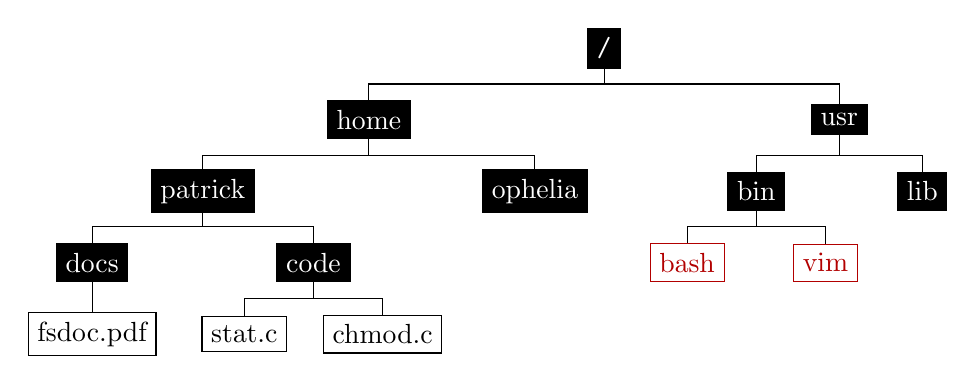
\begin{tikzpicture}[
  dir/.style={rectangle,draw,fill=black,text=white},
  file/.style={rectangle,draw},
  exe/.style={rectangle,draw=red!70!black,text=red!70!black},
  level 1/.style={sibling distance=17em,level distance=6ex},
  level 2/.style={sibling distance=5em,level distance=6ex},
]

\node [dir] {\verb|/|}
  [edge from parent fork down]
  child {node [dir] {home}
    child [sibling distance=12em] {node [dir] {patrick}
      child [sibling distance=8em] {node [dir] {docs}
        child {node [file] {fsdoc.pdf}}
      }
      child [sibling distance=8em] {node [dir] {code}
        child [sibling distance=5em] {node [file] {stat.c}}
        child [sibling distance=5em] {node [file] {chmod.c}}
      }
    }
    child [sibling distance=12em] {node [dir] {ophelia}}
  }
  child { node [dir] {usr}
    child [sibling distance=6em] { node [dir] {bin}
      child [sibling distance=5em] {node [exe] {bash}}
      child [sibling distance=5em] {node [exe] {vim}}
    }
    child [sibling distance=6em] {node [dir] {lib}}
  };
\end{tikzpicture}
\caption{File Hiearchy Tree}\label{fig:fstree}
\end{figure}
Figure \ref{fig:fstree} shows an example of how a (minimal) filesystem could be visualised. Black nodes in this tree represent directories, white nodes regular files and red nodes executable files. The difference between these will be examined in the next section. Getting the path to a file like \verb|stat.c| is done by simply joining all the names of the nodes on the path from the root to the file, in this case \verb|/home/patrick/code/stat.c|.

\subsection{Special Paths}

There are some conventions regarding special paths used to navigate directory hiearchies. The directory \verb|.| refers to the current directory, so in a path like \verb|/path/to/./file/|, the \verb|.| does not change the path. The \verb|..| however refers to the previous (upper) directory. Therefore, a path such as \verb|/path/to/other/dir/../../file| is equivalent to \verb|/path/to/file|.

Another convention is the special syntax for home directories. Specifying \verb|~patrick| refers to the home directory for the user \emph{patrick}, which is \verb|/home/patrick|. Specifying \verb|~root| refers to \verb|/root|, the home directory for the \emph{root} user, which is the highest-privileged user on \textsc{unix} systems.

% todo: lsmount util to list mounted?

% Every entry in the file hiearchy has an \emph{inode} number associated with it, uniquely identifying the file (entry).

\begin{table}
\begin{tabular}{@{}ll@{}}
\toprule
Path & Description\\
\midrule
\texttt{.} & Current directory\\
\texttt{..} & Parent directory\\
\texttt{\textasciitilde} & Home directory (of current user)\\
\texttt{\textasciitilde username} & Home directory (of username)\\
\bottomrule
\end{tabular}  
\end{table}


\subsection{Mounting}



\subsection{Changing Filesystem Root}

\subsection{Filesystem Hiearchy Standard}

There is a standard for file system hiearchies in Linux-like operating systems, called the \gls{fhs}. This is a document which is put forth by the \gls{lsb}, describing what Linux installations should look like filesystem-wise\cite{fhs3}. It has a mandatory directory structure, as well as some optional components. 

While this is an important document, illustrating how most Linux installations look like, not everyone sticks to these recommendations. For example, the NixOS distribution does not adhere to the \gls{fhs}, in order to provide isolation between packages\cite{vanderburg2011}. Debian, however, does follow the \gls{fhs} standard.

Figures \ref{fig:fhs1} and \ref{fig:fhs2} provide an overview of the directories required by the \gls{fhs}, and what their purpose is as described in the standard document.

\begin{figure}
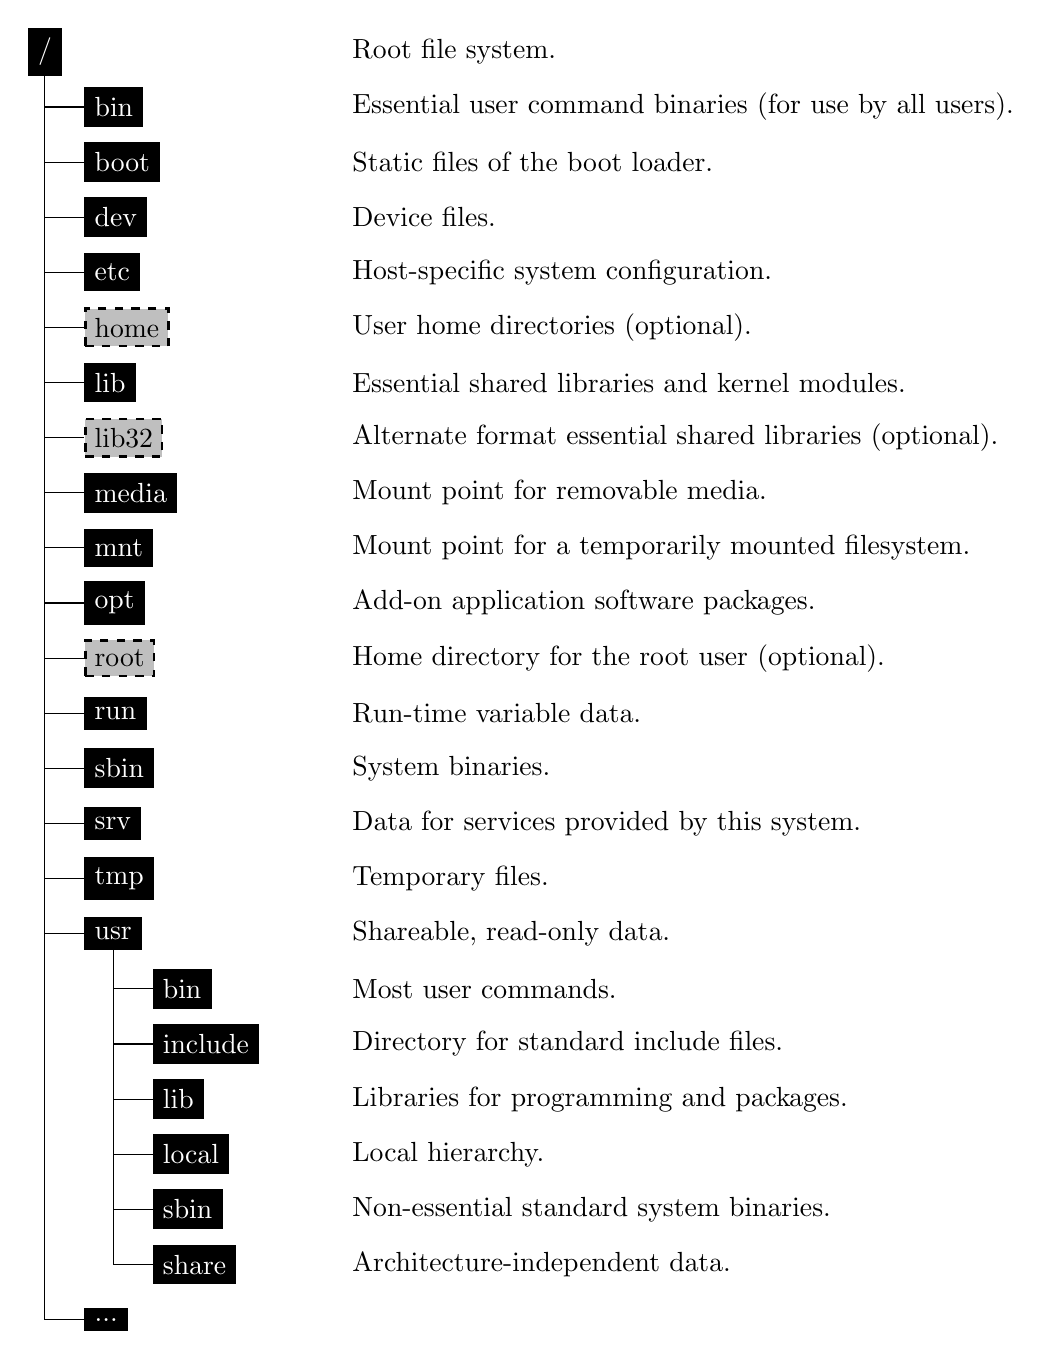
\begin{tikzpicture}[%
  dir/.style={draw=black,thick,anchor=west,draw=black,fill=black,text=white},
  opt/.style={draw=black,thick,anchor=west,dashed,fill=gray!50},
  desc/.style={anchor=west},
  grow via three points={one child at (0.5,-0.7) and
  two children at (0.5,-0.7) and (0.5,-1.4)},
  edge from parent path={(\tikzparentnode.south) |- (\tikzchildnode.west)}
]
  \node [dir] {/}
    child { node [dir] {bin}}
    child { node [dir] {boot}}
    child { node [dir] {dev}}
    child { node [dir] {etc}}
    child { node [opt] {home}}
    child { node [dir] {lib}}
    child { node [opt] {lib32}}
    child { node [dir] {media}}
    child { node [dir] {mnt}}
    child { node [dir] {opt}}
    child { node [opt] {root}}
    child { node [dir] {run}}
    child { node [dir] {sbin}}
    child { node [dir] {srv}}
    child { node [dir] {tmp}}
    child { node [dir] {usr}
      child { node [dir] {bin}}
      child { node [dir] {include}}
      child { node [dir] {lib}}
      child { node [dir] {local}}
      child { node [dir] {sbin}}
      child { node [dir] {share}}
      }
    child [missing] {}				
    child [missing] {}				
    child [missing] {}
    child [missing] {}
    child [missing] {}
    child [missing] {}
    child { node [dir] {...}};

\node at (4,    0) [desc] {Root file system.};
\node at (4, -0.7) [desc] {Essential user command binaries (for use by all users).};
\node at (4, -1.4) [desc] {Static files of the boot loader.};
\node at (4, -2.1) [desc] {Device files.};
\node at (4, -2.8) [desc] {Host-specific system configuration.};
\node at (4, -3.5) [desc] {User home directories (optional).};
\node at (4, -4.2) [desc] {Essential shared libraries and kernel modules.};
\node at (4, -4.9) [desc] {Alternate format essential shared libraries (optional).};
\node at (4, -5.6) [desc] {Mount point for removable media.};
\node at (4, -6.3) [desc] {Mount point for a temporarily mounted filesystem.};
\node at (4, -7.0) [desc] {Add-on application software packages.};
\node at (4, -7.7) [desc] {Home directory for the root user (optional).};
\node at (4, -8.4) [desc] {Run-time variable data.};
\node at (4, -9.1) [desc] {System binaries.};
\node at (4, -9.8) [desc] {Data for services provided by this system.};
\node at (4, -10.5) [desc] {Temporary files.};
\node at (4, -11.2) [desc] {Shareable, read-only data.};
\node at (4, -11.9) [desc] {Most user commands.};
\node at (4, -12.6) [desc] {Directory for standard include files.};
\node at (4, -13.3) [desc] {Libraries for programming and packages.};
\node at (4, -14.0) [desc] {Local hierarchy.};
\node at (4, -14.7) [desc] {Non-essential standard system binaries.};
\node at (4, -15.4) [desc] {Architecture-independent data.};
\end{tikzpicture}
\caption{File System Hiearchy: Example Filesystem Tree}\label{fig:fhs1}
\end{figure}

\begin{figure}
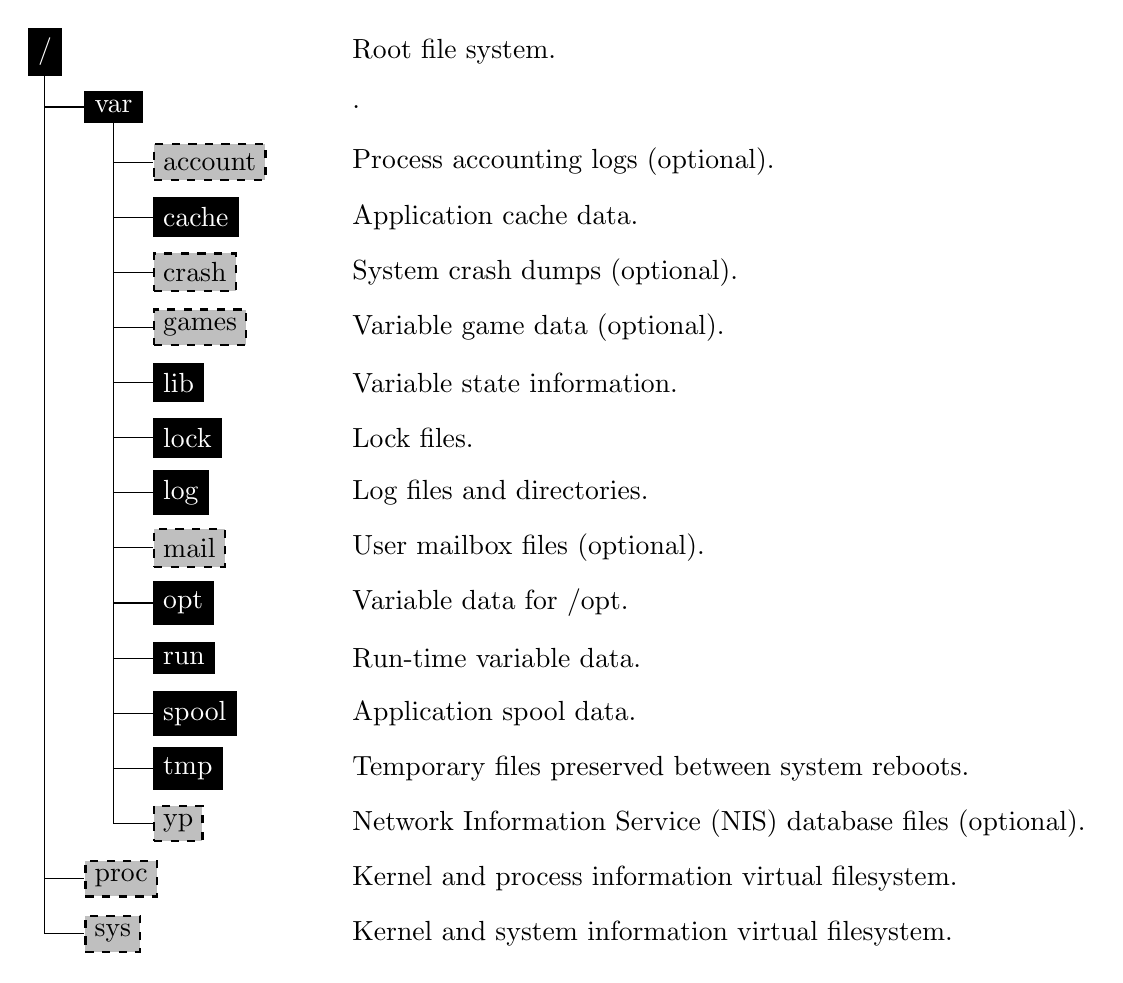
\begin{tikzpicture}[%
  dir/.style={draw=black,thick,anchor=west,draw=black,fill=black,text=white},
  opt/.style={draw=black,thick,anchor=west,dashed,fill=gray!50},
  desc/.style={anchor=west},
  grow via three points={one child at (0.5,-0.7) and
  two children at (0.5,-0.7) and (0.5,-1.4)},
  edge from parent path={(\tikzparentnode.south) |- (\tikzchildnode.west)}
]
  \node [dir] {/}
    child { node [dir] {var}
      child { node [opt] {account}}
      child { node [dir] {cache}}
      child { node [opt] {crash}}
      child { node [opt] {games}}
      child { node [dir] {lib}}
      child { node [dir] {lock}}
      child { node [dir] {log}}
      child { node [opt] {mail}}
      child { node [dir] {opt}}
      child { node [dir] {run}}
      child { node [dir] {spool}}
      child { node [dir] {tmp}}
      child { node [opt] {yp}}
      }
    child [missing] {}				
    child [missing] {}				
    child [missing] {}
    child [missing] {}
    child [missing] {}
    child [missing] {}
    child [missing] {}
    child [missing] {}
    child [missing] {}
    child [missing] {}
    child [missing] {}
    child [missing] {}
    child [missing] {}
    child { node [opt] {proc}}
    child { node [opt] {sys}};

\node at (4,    0) [desc] {Root file system.};
\node at (4, -0.7) [desc] {.};
\node at (4, -1.4) [desc] {Process accounting logs (optional).};
\node at (4, -2.1) [desc] {Application cache data.};
\node at (4, -2.8) [desc] {System crash dumps (optional).};
\node at (4, -3.5) [desc] {Variable game data (optional).};
\node at (4, -4.2) [desc] {Variable state information.};
\node at (4, -4.9) [desc] {Lock files.};
\node at (4, -5.6) [desc] {Log files and directories.};
\node at (4, -6.3) [desc] {User mailbox files (optional).};
\node at (4, -7.0) [desc] {Variable data for /opt.};
\node at (4, -7.7) [desc] {Run-time variable data.};
\node at (4, -8.4) [desc] {Application spool data.};
\node at (4, -9.1) [desc] {Temporary files preserved between system reboots.};
\node at (4, -9.8) [desc] {Network Information Service (NIS) database files (optional).};
\node at (4, -10.5) [desc] {Kernel and process information virtual filesystem.};
\node at (4, -11.2) [desc] {Kernel and system information virtual filesystem.};
\end{tikzpicture}
\caption{File System Hiearchy: Example Filesystem Tree, continued.}\label{fig:fhs2}
\end{figure}

\section{Entries}

A filesystem contains \emph{entries}. These are identified by the end user by a path such as \verb|/usr/local/bin/ruby|, where \verb|usr|, \verb|local| and \verb|bin| are \emph{directories} which form a hiearchy, and \verb|ruby| is a file. 

To the kernel, indidividual entries are identified by their \emph{inode} number, which typically is a 64-bit number. Every path (such as \verb|/usr/local/bin/ruby|), if it exists in the filesystem, resolved to an entry with an inode number. There can be multiple paths that have the same inode number. In that case, both paths refer to the same file, this is also known as a \emph{hard link}. Not all filesystems support hard links, notable \gls{apfs} does not support it.

% TODO insert citation about apfs and time machine.

It is possible to query the kernel for information (metadata) about an entry using the \verb|stat()| syscall. This returns a wealth of information, such as creation and access times, the inode number, and the entry type\footnote{For more information on this sycall, check \texttt{man 7 inode} and \texttt{man 2 stat}.}. 

In this project there is a utility, also called \verb|stat|, which uses this syscall and returns all information returned by the kernel. The output from calling this utility on \verb|~/.bashrc| looks like this.

\begin{verbatim}
$ stat ~/.bashrc
inode: 18785118
type:  regular
mode:  0644 (-rw-r--r--)
owner: 501 (pelsen)
group: 20 (staff)
links: 1
size:  17
atime: 2019-05-01T12:49:48Z
mtime: 2019-05-01T12:49:48Z
ctime: 2019-05-01T12:49:48Z
birth: 2019-05-01T12:49:48Z
dev:   1,4
rdev:  0,0
gen:   0
flags: 00000000 ()
\end{verbatim}
From the output of this utility we learn that the inode number of this particular file is 18785118. This is meaningful only to the filesystem. The type of this file is reported as a regular file. 

The permissions of this file are reported as 0644, this will be explored further in section \ref{sec:permissions} on page \pageref{sec:permissions}. Every entry also has an owner and a group associated with it. In this case, the file is owned by me, \gls{uid} 501.

The kernel reports how many (hard) links exist to this file. A file on the file system will have at least one link. It is possible, in Linux, to read from a file that has no links: a file is only fully removed when there are no links (entries in the filesystem to it) remain and it is not opened by any process anymore. It is thus possible to open and work with a file while another process deletes it. The behaviour here depends on the operating system, the “Windows” operating system for example does not support deleting files while they are opened by some process.

The size that is reported by the kernel is the file size in bytes. In the case of a regular file, it measures the length of data that is stored in the file.

The kernel reports four distinct times for this file. These are, in order of appearance, the \emph{access}, \emph{modification}, \emph{change}, and \emph{birth} times. The access time denotes the last time the file was accessed. On many systems, keeping track of this is disabled to reduce disk I/O and improve the longevity of hard drives. The modification time records the last time the contents of the file have been changed, such as by writing to it. The change time records the last time the file's status has changed, such as by changing its name or permissions. Lastly, the birth time records the time when the file was created. The Linux kernel does not support keeping track of the birth time.

% birth time seems to be a macOS-only feature?

% https://unix.stackexchange.com/questions/92816/can-a-file-be-retrieved-by-its-inode

\subsection{Directory}

A directory contains other entries. It can be created with \verb|mkdir| command. An empty directory can be deleted with \verb|rmdir|. Contents of a directory can be listed with the \verb|ls| command.

\begin{verbatim}
$ mkdir folder
$ rmdir folder  
\end{verbatim}
If a directory is not empty, it cannot be deleted with \verb|rmdir|.

\begin{verbatim}
$ mkdir folder
$ touch folder/file
$ rmdir folder
rmdir: failed to remove 'folder/': Directory not empty
\end{verbatim}
The \emph{stat} tool output of folders shows us that folders have the same metadata attached to them that regular files have.

\begin{verbatim}
  File: folder
  Size: 4096            Blocks: 8          IO Block: 4096   directory
Device: fc01h/64513d    Inode: 5680241     Links: 2
Access: (0775/drwxrwxr-x)  Uid: ( 1000/ patrick)   Gid: ( 1000/ patrick)
Access: 2019-09-26 13:49:04.481613173 +0000
Modify: 2019-09-26 13:49:09.853614507 +0000
Change: 2019-09-26 13:49:09.853614507 +0000
 Birth: -  
\end{verbatim}

The syscalls used to create, read and delete directories are \verb|mkdir()|, \verb|opendir()|, \verb|readdir()|, \verb|rewinddir()|, \verb|seekdir()|, \verb|telldir()|, \verb|scandir()|.

\subsection{Regular File}

Regular files are what we think of when we think of files. They contain data, and can be written to and read from.

\begin{verbatim}
$ echo hi > filename
$ cat filename
hi  
\end{verbatim}
The \emph{stat} tool output shows us that folders have a basic amount of metadata attached to them.

\begin{verbatim}
  File: file
  Size: 0               Blocks: 0          IO Block: 4096   regular empty file
Device: fc01h/64513d    Inode: 258817      Links: 1
Access: (0664/-rw-rw-r--)  Uid: ( 1000/ patrick)   Gid: ( 1000/ patrick)
Access: 2019-09-26 14:41:37.221013724 +0000
Modify: 2019-09-26 14:41:37.221013724 +0000
Change: 2019-09-26 14:41:37.221013724 +0000
 Birth: -
\end{verbatim}

Files can be created with the \verb|open()| sycall with the \verb|O_CREAT| flag, written and read to with \verb|write()| and \verb|read()|, and deleted with \verb|unlink()|.

\subsection{Symbolic Link}

Symbolic links are essentially files containing paths to the real file. When opening them, they act as a proxy to the real file. 

Syscalls used for creating and reading symbolic links are \verb|symlink()| and \verb|readlink()|.

\subsection{FIFO Queue}

\gls{fifo} queues are a type of special entry provided by the kernel. Unlike regular files, they don't store anything on disk. Rather, they are meant to be used by two processes, one process reading from it and the other writing to it. The data that is written is sent directly between these processes without being sent to disk first. Therefore, \gls{fifo} queues are a kind of \gls{ipc} mechanism.

\subsection{Socket}

Also called \textsc{unix} domain sockets, these are similar to network sockets in that they allow binding (listening for connections) and connecting, but without involving the network stack.

\subsection{Character Special File}

Character special files are entries that are handled completely by the kernel. They are identified by a pair of numbers, the minor and major number. Examples of this are \verb|/dev/null| and \verb|/dev/urandom|.

When reading or writing from them, the action that happens depends on their minor and major numbers in the kernel.

\subsection{Block Device}

A block device is very similar to a character special device, in terms of how it is used and the fact that it, too, is a kind of virtual file. Block devices are also handled completely by the kernel, and are typically used as an interface to hardware. For example, \verb|/dev/sda| is a block device, and is used for communicating to the raw storage of the first hard drive attached to the system. 

The actual difference between block- and character devices lies in the kernel. Character devices are devices that communicate on a byte basis, such as serial ports, whereas block devices communicate with blocks at a time. An example for this would be a hard drive, which has a native block size of, say, four kilobytes. The kernel can request a single block at a time. Therefore, reading from it is most optimal when done blockwise.

\section{Permissions}\label{sec:permissions}

UNIX sports a very simple permissions model that is based on a bitmask. Every file has an owner (user) and a group associated with it. The permissions that can be given are \emph{read}, \emph{write} and \emph{execute} for each of the owner, the group and the world (anyone). In addition to that, there is a set of special flags that can be set on entries, which are \emph{set-user-\textsc{id}}, \emph{set-group-\textsc{id}} and the \emph{sticky bit}.

These permissions are typically either shown in octal form (such as 0755) or in text form.

\begin{table}[!h]
\centering\caption{List of Permission Bits}
\begin{tabular}{@{}llll@{}}
\toprule
Name & Constant & Octal & String\\
\midrule
Owner read    & \verb|S_IRUSR| & 0400 & \verb|-r--------|\\
Owner write   & \verb|S_IWUSR| & 0200 & \verb|--w-------|\\
Owner execute & \verb|S_IXUSR| & 0100 & \verb|---x------|\\
\midrule
Group read    & \verb|S_IRGRP| & 0040 & \verb|----r-----|\\
Group write   & \verb|S_IWGRP| & 0020 & \verb|-----w----|\\
Group execute & \verb|S_IXGRP| & 0010 & \verb|------x---|\\
\midrule
Others read   & \verb|S_IROTH| & 0004 & \verb|-------r--|\\
Others write  & \verb|S_IWOTH| & 0002 & \verb|--------w-|\\
Others execute& \verb|S_IXOTH| & 0001 & \verb|---------x|\\
\midrule
Set \gls{uid} & \verb|S_ISUID| & 4000 & \verb|---s------|\\
Set \gls{gid} & \verb|S_ISGID| & 2000 & \verb|------s---|\\
Sticky bit    & \verb|S_ISVTX| & 1000 & \verb|---------t|\\
\bottomrule  
\end{tabular}
\end{table}
Permissions can be changed for files using the \emph{chmod} utility. An example of setting full read, write and execute permissions for owner, group and world might look like such.

\begin{verbatim}
$ touch file
$ chmod 0777 file
$ ls -l file
-rwxrwxrwx 1 patrick patrick 0 Sep 26 14:25 file  
\end{verbatim}
When removing read permissions, even the owner is unable to read from it.

\begin{verbatim}
$ touch file
$ chmod 0000 file
$ cat file
cat: file: Permission denied
\end{verbatim}

\subsection{Read}

The read permission is needed to open a file in reading mode. For directories, the read permission bit is needed to enumerate the contents with \verb|opendir()| and \verb|readdir()|.

\subsection{Write}

The write permission is needed to open a file in writing mode. For directories, the write bit is needed to create new entries into it.

\subsection{Execute}

The execute bit is needed to execute files as binaries. This is needed to run native binaries, but also shell scripts with a hashbang or anything that goes through the Linux kernel binfmt handlers.

% https://ownyourbits.com/2018/05/23/the-real-power-of-linux-executables/

The execute bit has a different meaning for directories. If it is not set, it is not possible to \verb|chdir()| into a directory.

\subsection{Set UID and Set GID}

The \verb|setuid| bit are special in the sense that they change the effective \gls{uid} and \gls{gid} of the running process. Normally, when running an executable, the \gls{uid} and \gls{gid} are set to that of the user that executes it.

\begin{verbatim}
$ ./perms
uid 1000 (patrick)
gid 1000 (patrick)
euid 1000 (patrick)
egid 1000 (patrick)  
\end{verbatim}
However, when the Set \gls{uid} bit is set, then the effective \gls{uid} is set to that of the user who \emph{owns} the executable, rather than the one who runs it.

\begin{verbatim}
$ chown root perms
$ chmod u+s perms
$ ./perms
uid 1000 (patrick)
gid 1000 (patrick)
euid 0 (root)
egid 1000 (patrick)  
\end{verbatim}
This functionality is used in executables that need extra capabilities but should be usable by non-root users as well. Examples for this are the \verb|/bin/ping| utility, which needs raw access to generate \gls{icmp} ping packets, or \verb|/usr/bin/sudo|, which grants superuser rights to regular users depending on its configuration.

However, since Linux kernel version 2.2, the capabilities granted to a superuser have been split up into more finer-grained capabilities, and using extended attributes, one can grant specific capabilities to executables without having to give it full superuser rights. This is recommended, but not done by most major Linux distributions.

\subsection{Sticky bit}

The sticky bit has an effect on directories only. When set, files in the directory can be deleted or renamed only by the owner of the file, or the owner of the directory. This is used for directories like \verb|/tmp|, where anyone should be able to write into, but files should not be able to be deleted by anyone other than the user that created them.

\section{Quotas}

Quotas allow the system to limit disk usage for certain individuals, groups or, as is the case on Linux, projects. This probably originated back in the time where servers were large and expensive and shared between many users, and were supposed to prevent users from using a disproportionate amount of system resources (disk space).

\subsection{User}

\subsection{Group}

\subsection{Project}

% https://lwn.net/Articles/623835/
% http://man7.org/linux/man-pages/man8/setquota.8.html

\section{Attributes}

Attributes are flags that can be set on filesystem entries. These attributes are, from what I can tell, not standardised across operating systems. 

\subsection{Linux}

Linux sports a number of attributes. Unlike macOS, where attributes are stored in a bitset that is returned with the \verb|stat()| syscall, in Linux a special \verb|ioctl()| call has to be used to access and set them.

% man chattr
% man ioctl_iflags

\subsubsection{Append-only file}

The xxx.

\subsection{MacOS}

% help: what is https://ss64.com/osx/setfile.html setfile? 
% what does it do and how does it work?

% how are these flags different from attrs like getattrlist
% and setattrlist?

MacOS also supports file attributes, called \emph{flags}. They are returned as a bitmask in the \verb|sv_flags| field of the \verb|stat()| syscall. The \verb|stat| utility included in this project displays the flags set for a given file by using the system-provided \verb|fflagstostr()| function to decode the bitmaks to a comma-delimited string.

\begin{verbatim}
$ stat /bin | grep flags
flags: restricted,hidden
\end{verbatim}
Table \ref{tbl:macosflags} lists all flags currently known to and implemented in the MacOS kernel, as of the time of writing\footnote{\texttt{/Library/Developer/CommandLineTools/SDKs/MacOSX.sdk/usr/include/sys/stat.h} documents the currently known and used flags.}. Some flags (those beginning with \verb|SF_|) are limited in that they can only be set by the superuser, and while \gls{sip} is active, additional restrictions apply when setting or clearing certain flags. 
\begin{table}
\centering\caption{MacOS File Attributes (Flags)}\label{tbl:macosflags}
\begin{tabular}{@{}lllp{5cm}@{}}
\toprule
Name & Constant & Value (hex) & Description\\
\midrule
\emph{nodump} & \verb|UF_NODUMP| & 00\,00\;00\,01 & Don't dump this file.\\
\emph{uchg} & \verb|UF_IMMUTABLE| & 00\,00\;00\,02 & Immutable.\\
\emph{uappnd} & \verb|UF_APPEND| & 00\,00\;00\,04 & Append-Only.\\
\emph{opaque} & \verb|UF_OPAQUE| & 00\,00\;00\,08 & Opaque in union mount.\\
— & \verb|UF_COMPRESSED| & 00\,00\;00\,20 & Compressed.\\
— & \verb|UF_TRACKED| & 00\,00\;00\,40 & Tracked.\\
— & \verb|UF_DATAVAULT| & 00\,00\;00\,80 & Datavault.\\
\emph{hidden} & \verb|UF_HIDDEN| & 00\,00\;80\,00 & Hidden from \glsname{gui}.\\
\midrule
\emph{arch} & \verb|SF_ARCHIVED| & 00\,01\;00\,00 & Archived.\\
\emph{schg} & \verb|SF_IMMUTABLE| & 00\,02\;00\,00 & Immutable.\\
\emph{sappnd} & \verb|SF_APPEND| & 00\,04\;00\,00 & Append-Only.\\
\emph{restricted} & \verb|SF_RESTRICTED| & 00\,08\;00\,00 & File is under \glsname{sip}.\\
\emph{sunlnk} & \verb|SF_NOUNLINK| & 00\,10\;00\,00 & Undeletable.\\
\bottomrule  
\end{tabular}
\end{table}
Apple's \gls{sip} uses the \emph{restricted} flag to mark files and folders as system folders, which cannot be set or unset by anyone unless \gls{sip} is turned off.

It is possible, on macOS, to view the file attributes using \verb|ls| with the \verb|O| flag. 

\begin{verbatim}
$ ls -oOd /bin /Volumes /net /private
drwxr-xr-x+  4 root  hidden             128 Sep 25 20:11 /Volumes
drwxr-xr-x@ 37 root  restricted,hidden 1184 Jun 12 15:54 /bin
dr-xr-xr-x   2 root  hidden               1 Sep 24 09:31 /net
drwxr-xr-x   6 root  sunlnk,hidden      192 Sep 27  2018 /private  
\end{verbatim}

% https://en.wikipedia.org/wiki/File_attribute

\subsubsection{Nodump}

The \emph{nodump} flag can be set by any regular user and signals to the \emph{dump} utility, which was used for backups in old versions of \textsc{unix} and is long obsolete, that this file should not be included in the dump. This flag has no effect on file operations and is merely a signal to other applications.

\subsubsection{Immutable}

The \emph{uchg} and \emph{schg} flags disable any kind of modification from being done to a file with this flag. That includes writing to it, renaming it, and deleting it. 

\begin{verbatim}
$ flags file uchg
$ echo hi > file
-bash: file: Operation not permitted
$ echo hi | sudo tee file
tee: file: Operation not permitted
$ unlink file
file: Operation not permitted
$ flags file nouchg
$ unlink file
\end{verbatim}
While their effects are identical, the difference between these flags is that the \emph{uchg} flag can be set and cleared by the owner of the file, whereas the \emph{schg} flag can only be set and cleared by the superuser.

\begin{verbatim}
$ chflags schg file
$ echo hi > file
-bash: file: Operation not permitted
$ echo hi | sudo tee file
tee: file: Operation not permitted
$ unlink file
file: Operation not permitted
$ sudo chflags noschg file
$ unlink file
\end{verbatim}

\subsubsection{Append-Only}

The \emph{uappnd} and \emph{sappnd} flags prevent a file from being overwritten, by only letting processes open it in append mode. It also prevents the file from being deleted with \verb|unlink()|, renamed or hard links to it being created. The difference between the two is that \emph{uappnd} can be set and unset by the owner, whereas \emph{sappnd} can only be set and unset by the superuser.

\begin{verbatim}
$ touch file
$ flags file uappnd
$ echo hi > file
-bash: file: Operation not permitted
$ echo hi >> file
\end{verbatim}

\subsubsection{Opaque}

The opaque flag plays a role when using a union mount. This happens when mounting a filesystem over another filesystem such that both are visible. When setting the opaque flag on a directory, then this union property does not work for the directory.

% TODO: example of a union mount.

\subsubsection{Hidden}

The hidden flag hides files or folders that it is defined on from the GUI. 

\begin{figure}
\centering\caption{Hidden Makefile}\label{fig:macoshidden}
\includegraphics[width=12cm]{img/hidden}  
\end{figure}

\begin{verbatim}
$ ls
Makefile  fsdoc.tex src
$ flags Makefile hidden
$ open .
\end{verbatim}
See Figure \ref{fig:macoshidden} to see that the Makefile is indeed hidden from Finder.

\subsubsection{Archived}

The archived flag is not handled by the kernel itself. It can be set to mark that a file has been archived, such as during a backup operation. This flag has no effect on file operations.

\subsubsection{Restricted}

\subsubsection{Nounlink}

\subsubsection{Tracked}

\subsubsection{Compressed}

\subsubsection{Datavault}

\subsubsection{Undocumented}

Not every bit in the bitfield has a name. Undocumented bits can still be set, but they have no effect. This can be used to store data. Experimenting shows that a bitmask of \verb|7F00| are bits that can be set by users that are not filtered by the system and at the same time have no effect, thus they can be used to store some information in a way that is not obvious.

\section{Extended Attributes}

Extended Attributes allow storing of arbitrary metadata of files on a file system. The concept of them was from the \gls{posix}\.1e draft which was withdrawn.

% https://unix.stackexchange.com/questions/489820/why-was-posix-1e-withdrawn

% https://git.kernel.org/pub/scm/linux/kernel/git/torvalds/linux.git/tree/include/uapi/linux/limits.h

The amount and size of attributes that can be set depend on the filesystem. Some filesystems, such as \gls{fat}, do not support them at all, while others like the \gls{ext} family of filesystems limit them.

POSIX Extended Attributes are divided into different namespaces. The \emph{user} namespace has no restrictions on what attributes can be set. 

\subsection{Capabilities}

\subsection{Access Control Lists}

\gls{acl} is a feature by which access to filesystem entries can be controlled more finely than with UNIX permissions\footnote{See \texttt{man acl} for more information}.


\section{Alternate File Streams}

\subsection{HFSs+ Resource Fork}

A resource fork is a section of a file besides the file's actual contents that can be used to store structured data besides the unstructured data of the file itself. They appear as the extended attribute \verb|com.apple.ResourceFork|. 

Apple has a special syntax that can be used to access these forks with the standard \gls{posix} \gls{api} and tools. Given a file \verb|filename|, the special path \verb|filename/..namedforks/rsrc| can be used to access the resource fork.

\begin{verbatim}
$ touch file
$ echo hi > file/..namedforks/rsrc
$ cat file
$ cat file/..namedforks/rsrc
hi  
\end{verbatim}

Using \verb|ls -l@|, the extended attributes of the file can be listed, revealing the resource fork attribute.

\begin{verbatim}
$ ls -l@ file
-rw-r--r--@ 1 pelsen  staff  0 Sep 27 22:49 file
        com.apple.ResourceFork  3  
\end{verbatim}

These resource forks are a feature carried over from classic MacOS, and are not really used anymore. In fact, the \gls{api} to access them, \emph{Resource Manager}, have been removed. There are, to the best of my knowledge, no other named forks apart from the resource fork exposed.

\subsection{NTFS Alternate Data Streams}

% https://www.borncity.com/blog/2018/09/22/infos-zu-windows-ntfs-alternative-data-streams/

\gls{ntfs} supports alternate data streams, which are used by Microsoft to tag downloaded files as being unsafe. It is also an interesting way to hide malware.

\section{Locks}

File locking is supported with the \verb|flock()| syscall.

% TODO: example, writeup.

\section{Virtual Filesystems}

% TODO: introduction, comparison to /dev, justification, some history.

\subsection{Proc}

% TODO: overview, examples.

\subsection{Sys}

% TODO: overview, examples.

\section{\glsdesc*{fuse}}

\gls{fuse} is a facility by which filesystems can be implemented in userspace, meaning that requests are proxied from the kernel into a userspace process. Unlike regular filesystems, which are implemented and run in the kernel. This has some advantages, namely that a user does not need superuser privileges to mount a userspace filesystem, and it also means that an experimental filesystem can be quickly hacked up and played around with without running the change of causing the kernel to crash, as a misbehaving regular filesystem might do. 

On the other hand, \gls{fuse} filesystems also have a number of restrictions. Features like the \emph{setuid} bit or the capabilities that extended attributes allow setting on executables mean that if an unprivileged user can fully control a filesystem, a system can be easily compromised. For this reason, \gls{fuse} filesystems are more limited.

\printglossaries

\printbibliography

\end{document}